%\documentclass[aps,pra,reprint,longbibliography]{revtex4-1}
\documentclass[twocolumn]{article}

\usepackage{geometry}
\geometry{textwidth = 18cm,textheight = 24cm}

%\usepackage{multicol}
\usepackage{cite}
\usepackage{caption}
\usepackage{graphicx}
\usepackage{amsmath}
\usepackage{float}
%\usepackage{amssymb}
\usepackage{textcomp}
\usepackage{lmodern}
\newenvironment{figure_alt}
  {\par\medskip\noindent\minipage{\linewidth}}
  {\endminipage\par\medskip}

\begin{document}
	
	%-------------------- begin header -------------------%
	\centerline{\LARGE Optoelectronic Neural Systems}
	\vspace{0.5em}
	\centerline{\Large Device and Architecture Considerations}
	\vspace{0.25em}
	\centerline{\Large for General Intelligence}
	\vspace{0.75em}
	\centerline{\large Jeffrey M. Shainline}
	%\vspace{0.75em}
	%\centerline{\large National Institute of Standards and Technology}
	\vspace{0.5em}
	\centerline{\normalsize NIST, Boulder, CO, 80305}
	\vspace{0.5em}
	\centerline{\small \today}
	%-------------------- end header ---------------------%
	
\begin{abstract}

\end{abstract}

\tableofcontents

\section{\label{sec:introduction}Introduction}
Optoelectronic neural systems reside at the confluence of multiple disciplines. The subject is derived in large part from the foundations of communication theory and computation, as established by Turing \cite{tu1936}, von Neumann \cite{ne1945}, Shannon \cite{sh1948} and others. Yet the nature of information processing in neural systems is not wholly captured by the mathematical analysis formalized to describe serial communication and computation of digital signals. Concepts from neuroscience dating back to Ramon y Cajal \cite{}, Mountcastle \cite{}, Edeleman \cite{}, and many others during the flourishing of the last 40 years indicate that clean, serial data streams have much to gain from the network concepts of neural systems with complex spatial and temporal behavior, particularly if one seeks a machine that can think like an intelligent being. If one seeks complexity of performance, one must provide complexity in hardware. If one seeks comprehension in the face of ambiguity, the computation must be able to handle shades of gray. Probability and statistics are inherent to neural systems. 

Conceptually, neural systems contain threads of communication theory, digital logic, probability and statistics. In practice, these systems combine the physics of many devices. The systems envisioned here utilize electrons to compute and photons to communicate. They leverage semiconductors to make light and superconductors to compute. At this confluence of physics and computing, it is possible to conceive of systems with complexity from the chip scale to the globe, employing the logic of neural systems for cognitive information processing across broad reaches of space and time. 

Why do this now? Why this way? Since the inception of the EDVAC, its limitations were anticipated \cite{}. Yet the microelectronic march delayed the consequences by many decades. The scaling first charted by Moore \cite{} left little impetus for revolutionary concepts. Now that scaling is reaching physical limitations \cite{}, there is an appetite for what new hardware may have to offer. And as computing machines have become deeply integrated in society, we are ready for a sea change in what we ask our machines to do. They can answer any question of fact, but that is no longer all we ask of them. We seek intelligent machines, computers that think, not superficially, but with as deep a wisdom as we can manage to construct. That is why we seek to combine the strengths of superconductors and light. In conjunction, we think, they will lead to the most intelligent machines. To put this discussion in context, we must revisit the origins of computing.

\section{\label{sec:history}Historical context}
Much of nature is best described by analog values. The radius of a planet's orbit can take any value across a broad range. The light output from a star is a smoothly varying function. Yet upon close inspection, that light is discrete. A photon is either there, or it is not. The ancient Chinese saw such dichotomies as central to the balance of nature, represented symbolically in the yin-yang. This concept led them to invent binary arithmetic as a representation of the interaction between mutually interdependent opposites \cite{http://www.atimes.com/leibniz-chinese-invented-first-binary-code/}. Francis Bacon extended these ideas in 1623 to establish that two symbols were sufficient for encoding any communication \cite{dy2012}, a concept that was matured by Claude Shannon during and after WWII \cite{sh1948}. Bacon was also well aware 400 years ago that optical communication was advantageous for such communication, although he probably did not anticipate the complex fiber-optic networks that now span the globe. Leibniz further developed these ideas \cite{http://www.leibniz-translations.com/binary.htm} with the intention to utilize binary arithmetic for computing \cite{https://hal.archives-ouvertes.fr/ads-00104781/document,dy2012}. In 1679, Leibniz proposed a mechanical apparatus for digital computing based on marbles passing through holes to perform logical operations. 

From the earliest intellectual explorations into the digital domain, it has been clear that one of the great strengths of digital information processing is the simplicity of the binary format. Information provides the ability to answer questions, and a bit allows one to answer a single question. This or that? Yes or no? Yet despite the simplicity, a more rigorous mathematical foundation (provided by Alan Turing) as well as the motivations of war would be required before the Leibniz's vision of a digital computer would be realized.

In 1936, Turing published his seminal work ``On Computable Numbers'' \cite{tu1936}, wherein he introduced the concept of a universal computing machine that, provided sufficient time and memory, could execute any computation that is possible, in principle, within the framework established by G\"{o}del \cite{}. Turing's contribution was of fundamental mathematical importance in that it further strengthened the arguments made by G\"{o}del regarding the existence of unsolvable problems (the ``entscheidungsproblem'', as laid out by Hilbert), but Turing's contribution was also of practical importance in that it provided a specific vision for the realization of a universal computer. Turing would go on to design a hardware manifestation of such an apparatus, but his system would never be built. Like the ancient Chinese, Bacon, Leibniz, Babbage, and many others to come, Turing was convinced of the necessity of implementing computation with binary symbols. As he stated in 1947, ``Being digital should be of more interest than being electronic.'' \cite{tu1947} 

Turing's work on decrypting messages encoded by the enigma machine during WWII led to advances in computing hardware, in part by leading to the construction of Colossus, a British machine used for analyzing wartime communications, but also by the influence Turing's ideas had on John von Neumann. Von Neumann appreciated the significance of Turing's universal computer, both for the insights regarding issues of completeness raised by G\"{o}del, and also for the utility of enabling a single machine to be capable of performing any possible calculation. During the war, von Neumann found it imperative that the United States develop an atomic weapon, and he appreciated the necessity of numerically modeling various aspects of the detonation of nuclear weapons. Beginning with the Manhattan Project in Los Alamos, and continuing at the Institute for Advanced Study at Princeton after the war, von Neumann was dedicated to creation of universal calculators in the mold of a Turing machine, the objective being to numerically analyze arbitrary differential equations, represented as difference equations with binary arithmetic. This objective led to the construction of apparatus with a centralized computing unit that could follow arbitrary (clearly articulated) instructions, and could read and store information in a separate memory unit. The memory unit could contain initial conditions, the results of calculations, and instructions that could be modified during the execution of the computation. 

In 1953, a machine at the Institute for Advanced Studies employing this ``von Neumann'' architecture was primarily used for five types of calculations: nuclear explosions, shock waves, meterology, biological evolution, and stellar evolution. Already at that time, the universal machine was analyzing problems across 25 orders of magnitude in time and roughly the same number in space. During the subsequent 70 years, the von Neumann architecture has been used to answer questions regarding essentially every conceivable subject of any concern whatsoever to human beings. This trajectory represents tremendous success regarding von Neumann's initial goal. Nearly all modern computing is based on digital (binary) information processed in a von Neumann architecture, a scheme devised as a means to realize a Turing machine in electronic hardware. 

Over the course of this time, hardware for computation has shifted from vacuum tubes, in which information is represented by the deflection of an electron beam under the influence of a voltage, to silicon microelectronics, in which information is represented by the flow of electrical current through a transistor under the influence of a voltage. This evolution of hardware has been perhaps as important as the original conception of the architecture  in terms of enabling sustained technological evolution. While hardware has advanced tremendously, the underlying concepts regarding the form of computation performed have remained relatively static. In particular, two key traits of the von Neumann architecture have descended to this day from Turing ancestry: serial information processing, and separation of computation and memory. 

John von Neumann would likely be surprised by the constancy of the architecture. As he stated in 1949, ``There is reason to suspect that our predilection for linear codes, which have a simple, almost temporal sequence, is chiefly a literary habit, corresponding to our not particularly high level of combinatorial cleverness, and that a very efficient language would probably depart from linearity.'' \cite{ne1949} Von Neumann did not see the sequential processing performed by Turing's original conceptual apparatus as an ideal way to go about computing, but rather as a convenient way to get started, and certainly a useful tool for numerical investigation. Other limitations of the Turing machine and von Neumann architecture were also well known shortly after their conceptions. Julian Bigelow, the chief engineer of the Electronic Computer Project at the Institute for Advanced studies, articulated that, ``If you actually tried to build a machine the way Turing described it, you would spend more time rushing back and forth to find places on a tape than you would doing actual numerical work or computation.'' Regarding the von Neumann architecture as implemented with vacuum tubes, Bigelow commented, ``The design of an electronic calculating machine...turns out to be a frustrating wrestling-match with problems of interconnectivity and proximity in three dimensions of space and one dimension of time.'' Integrated silicon microelectronics enabled tremendous advances in computer, in large part because of the ability of lithographically defined wires to achieve extraordinary interconnectivity. Yet the challenges of routing information through space and time still form the core motivation for pursuing neural systems with optical interconnectivity.

Beyond hardware constraints, those at the dawn of electronic computation identified logical limitations as well. Describing generations of computers following the EDVAC, Bigelow stated, ``The modern high speed computer, impressive as its performance is, from the point of view of getting the available logical equipment adequately engaged in the computation, is very inefficient indeed.'' Von Neumann went further, beginning to articulate his vision for new types of logic for computation. He claimed, ``Whatever language the central nervous system is using, it is characterized by less logical and arithmetical depth than what we are normally used to.'' \cite{ne1958} Von Neumann anticipated the highly parallel computation performed by neural systems, and was likely influenced by the work of McCulloch and Pitts nearly a decade prior. In 1943, they showed that perceptrons (devices with computational properties loosely based on the nonlinear behavior of neurons in the brain) could be used to represent any logical expression, much like universal computation performed by a Turing machine \cite{mcpi1943}. 

While some were conceiving of how to utilize principles of neural information processing for computation, Alan Turing was contemplating whether any artificial machine could eventually embody the intelligence demonstrated in the brain. In 1950, Turing published ``Computing Machinery and Intelligence'', in which he argued that artificial intelligence should indeed be possible, and he offered a means to determine if it had been achieved, now referred to as the Turing Test \cite{tu1950}. After 70 years of development of hardware, with devices now defined at the nanometer scale, and architectures such as RISC-V that standardize instructions across Turing machines, silicon microelectronic hardware still appears far from achieving general intelligence. Turing was interested from the beginning in constructing a machine that could think, but the Turing Machine as originally conceived is not adept at the task. A silicon digital supercomputer can provide the answer to very hard math problems, and it can search databases, route information over switching networks, and control robots and automobiles. But such an architecture is not conducive to forming a broad concept of what is going on in the world. The digital system struggles with context, with the inter-relations between quantities. It is the intelligence Turing was attempting to emulate that is most difficult to achieve artificially with the serial operation of the Turing machine. 

To achieve the intelligence of a human being, we must depart from the serial operation of a Turing machine, we must step away from the framework of the von Neumann architecture, and we must begin to speak in languages beyond binary. As expressed by von Neumann, ``A new, essentially logical, theory is called for in order to understand high-complication automata and, in particular, the central nervous system. It may be, however, that in this process logic will have to undergo a pseudomorphosis to neurology.'' \cite{ne1951} This statement in 1951 anticipates the development of neuromorphic computing in calling for a form of complex information processing modeled after neural systems. After his untimely death in 1958, little effort was made to pursue this vision. As historian George Dyson explains, ``The reliability of monolithic microprocessors and the fidelity of monolithic storage postponed the necessity for this pseudomorphosis far beyond what seemed possible in 1948.'' \cite{dy2012} The extraordinary success of silicon technology has made innovation in architecture and logic lack urgency.

The aspirations to achieve general intelligence and to incorporate the processes of the brain to enable new forms of computing have persisted. In 1990, Carver Mead introduced the concept of using silicon transistors to perform the operations of neurons \cite{me1990}. Mead's idea was not to use digital logic to numerically step through the differential equations describing neurons, but rather to use the physics of transistors in the sub-threshold regime to embody an approximation of the dynamics inherent to neuronal operation. Such an approach operates MOSFETs as analog integrators. This idea has been important conceptually to establishing the field of neuromorphic computing, but in practice it has been difficult to achieve high performance, due in part to the challenge of achieving consistent performance from analog devices, the same challenge that led to the victory of digital over analog computing for numerical analysis. 

Nevertheless, Mead's perspective marked the beginning of a trend that has been exponential since. The majority of the field of neuromorphic computing at present attempts to combine the silicon hardware that has been so successful with the highly parallel, spike-based computation that is observed in biological neural systems. The goal is to use hardware that can be manufactured economically at large scale to implement the new logic von Neumann anticipated when vacuum tubes were still in use. In this paper we argue that such hardware is not well equipped for neural information processing, but that with a different use of silicon microelectronic manufacturing, new devices and systems can be achieved economically that are tailored to this form of computation. Turing and von Neumann did not live to see the silicon revolution, nor were they privy to insights from modern neuroscience. From the perspective of the present day, we are in a much better position to design technologies that speak the language of the human brain to achieve the vision of machines that think.

%At present, work in in the field of neural computing is largely divided into two categories. One category involves creation of devices that perform neural functions, such as establishing synaptic weights or achieving relaxation oscillations like a spiking neuron. The other category 
 
\vspace{4em}
Turing/von Neumann/digital: I'm going to give you these instructions and this input. I want you to generate an output that is the one and only (existence and uniqueness theorem) correct answer to a mathematically well-posed question.

brain/AGI: I'm going to give you an enormous amount of information regarding the world and all its parts. I want you to distill the essence, identify the salient relationships, and conceive of it all simultaneously across various spatial and temporal scales. And I want you to explain this world to me.

These are very different objectives. A Turing machine is a universal computer in the sense that if a procedure exists to calculate a given number, a Turing machine can do it. However, two aspects of the Turing model make it inefficient for the latter task. First, information processing is serial. Second, memory must be accessed as an independent step from change of internal state (processing).

\section{\label{sec:neuroscience}Information processing in neural systems}
Information processing in a Turing machine is a serial operation. The state of the machine is updated in a sequential manner based on instructions and the contents of memory. Neural computation departs markedly from this approach. Enormous numbers of operations in the brain occur simultaneously, with many neurons receiving communications from many neighbors and independently accessing local synaptic memory. The essence of neural information is to share the burden of computation across a large network of processors, while connecting them and signaling in such a way to enable the information of the disparate elements to be efficiently integrated in system-wide operations. Where a bit in a digital system enables one to answer a single binary question, the large number of synapses input to a neuron enable one to answer a large number of simple analog questions. Whereas the von Neumann architecture requires external memory to be read and written at each computational step, processing and memory are not distinct in neural systems. Whereas digital computing with a Turing apparatus can integrated information from separate calculations in a serial manner, neural information is, by its nature, integrated across a spatial and temporal hierarchy.

Perhaps the key concept behind neural cognition is the ability for systems to achieve differentiated local processing combined with information integration across space and time. Each neuron is receptive to a certain subset of information, and it will pulse in response to presentation of that information, while remaining quiescent under other stimuli. The response of the neurons in a network is differentiated, so they each express different signals, yet a simultaneous interpretation of a broad array of information can be gained through the network as a whole. 

\subsection{Spatial structure of neural systems}
\subsubsection{Adjacency matrix}
In order for the neurons to differentiate their responses while efficiently exchanging information across the network, certain structural network considerations are pertinent \cite{rusp2010}. The structures of neural systems are analyzed in the framework of network theory \cite{eskn2015}. In network theory, a system is discussed as a set of nodes connected by a set of edges. To facilitate mathematical analysis, the system is represented by an adjacency matrix, $\mathbf{A}$. Each column of $\mathbf{A}$ represents a node in the network, and if an edge connects node $i$ to node $j$, $A_{ij} = 1$, otherwise $A_{ij} = 0$. Connections can be directed, in which case $\mathbf{A}$ will be, in general, non-symmetric. Connections can also we weighted, in which case the adjacency matrix becomes a weight matrix, $\mathbf{W}$, whose elements represent not only the presence of edges, but also their strength.

To analyze a network, we label each node with an index $1\le i\le N$, where $N$ is the total number of nodes in the network. If we know all the connections between the nodes in the network, we can proceed to construct the adjacency matrix. In neural systems, we may use network theory to analyze the system at various scales. At the smallest (device) scale, each neuron may be represented a node, and each synapse by a directed edge. Alternatively, at the system scale, brain regions may be represented by nodes and the connections between these regions by edges. Across these scales, certain network metrics are important for analyzing performance. 

\subsubsection{Node degree and degree distribution}
A simple yet important quantity that can be calculated from the adjacency matrix is the number of connections made by each node. If the network has directed connections, the number of outgoing edges (out-degree) will, in general, be different from the number of incoming edges (in-degree). The out-degree is given by $k^{\mathrm{out}}_i = \sum_jA_{ij}$, and the in-degree is given by $k^{\mathrm{out}}_j = \sum_iA_{ij}$. At the scale of devices, the in-degree represents the number of synaptic connections terminating on a given neuron, and the out-degree represents the number of synaptic connections made by a given neuron. The function describing the degrees of all nodes in network is referred to as the degree distribution.

\subsubsection{Path length}
One reason the node degree is important is that it enables us to calculate the average minimum path length across the network. To calculate this quantity, we find the minimum path length (number of edges that must be traversed) for each pair of nodes in the network, and we take the average over all pairs. This average minimum path length is a coarse, global metric that provides information regarding the ability of information to be efficiently exchanged across the network. In constructing a neural system, one would like to keep path lengths as short as possible to facilitate efficient communication from any neuron to any other neuron. In general, network path lengths are minimized in random networks \cite{baal1999}, wherein edges between nodes are assigned at random. Therefore, by considering the average minimum path length of a random network, we can estimate the connectivity required between neurons in order to maintain efficient communication across a neural system of a given size. This average path length can be calculated in closed form \cite{frfr2004}. This quantity is plotted in Fig.\,\ref{fig:data}(a), where we show the number of edges required per node ($\bar{k}$) to achieve a given average path length ($\bar{L}$) as a function of the number of nodes in the network \cite{frfr2004}. Consider the case of a network with one million nodes. We see from this plot that if we wish to maintain a path length of two, each node must make, on average, one thousand connections. For the case of a network with 100 million nodes, each node must make 10,000 connections. This is similar to the case of the hippocampus in the human brain, with nearly 100 million neurons, each with 10,000 or more synaptic connections \cite{bu2006}. Maintaining a short average path length across the network is critical to enable efficient information integration, and this appears to be a major factor driving the extensive connectivity of biological neural systems, and our design of neural hardware for cognition must account for the requirement of many connections to enable efficient communication across the network.  
\begin{figure} 
    \centering{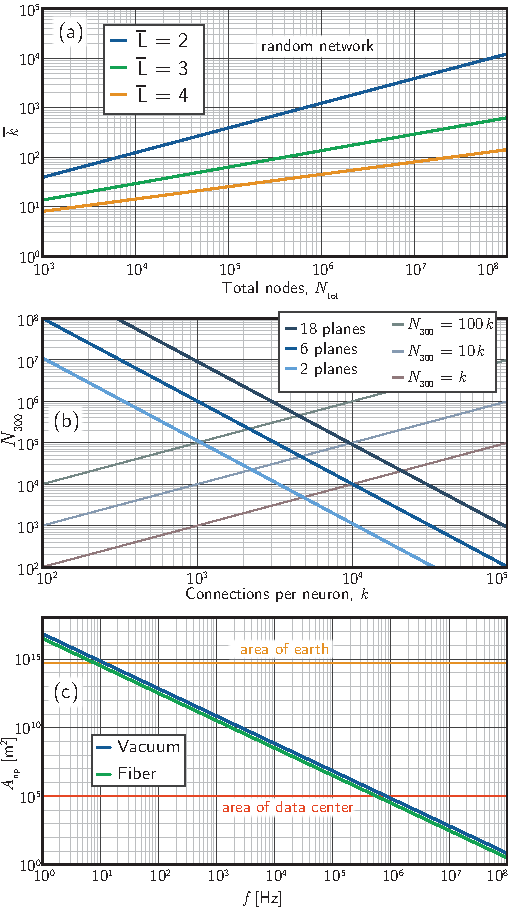
\includegraphics[width=8.6cm]{data_plots.pdf}}
	\captionof{figure}{\label{fig:data}Scaling considerations for optoelectronic neural systems. (a) The average number of connections per node required to maintain a give average path length across a random network as a function of the total number of nodes in the system. (b) The total number of nodes that can fit on a 300\,mm wafer as a function of the number of connections per node in the wire-limited regime \cite{ke1982}. (c) The area of the neuronal pool as a function of the frequency of neuronal oscillations assuming light-speed communication \cite{shICRC2018}.}
\end{figure}

\subsubsection{Clustering}
This analysis of average path length is relevant for quantifying a network's potential for information integration, but as we stated above, a neural system also depends on the ability for differentiated processing. Let us consider differentiation across various scales of the network. Ideally, no two neurons would behave identically, because this would not provide new information. Each neuron will fire preferentially in response to stimulus according to a tuning curve \cite{daab2001}. In practice, some redundancy is advantageous if a network is to rapidly gain confidence regarding the nature of a stimulus. Neural systems employ populations of neurons to represent certain pieces of information. The net activity across the population represents the presence or absence of a stimulus, and the variation in activity across the population represents uncertainty about the interpretation of the stimulus. In order for a certain population of neurons to predominantly exchange information locally and rapidly establish a consensus interpretation of a stimulus, the neurons in that population should comprise a preponderance of connections within the population. Groups of neurons with an abundance of connections within the group relative to connections external to the group form a community, and a clustering coefficient \cite{eskn2014,fa2007} is the simplest network metric. If node $a$ is connected to node $b$ and to node $c$, the clustering coefficient quantifies the fraction of cases in which node $b$ is also connected to node $c$. This metric provides insight into the tendency of neurons to form specialized communities with information processing differentiated from other parts of the network, and is first step toward analyzing the modularity of the system. 

\subsubsection{Small-world networks}
A random network has a low clustering coefficient, as the presence or absence of a connection between nodes $b$ and $c$ is, by definition, completely independent of the presence or absence of any connections to or from node $a$. Yet the networks of the brain\textemdash from the scale of neurons to the scale of connections between regions\textemdash show a high degree of clustering relative to a random network. As we have emphasized, neural information processing relies on both differentiated processing by local clusters and efficient integration of information across the network. We therefore expect neural systems to simultaneously achieve a high clustering coefficient and short average path length. A small-world networks is one with both of these traits \cite{wast1998}. We can introduce the small-world index (SWI) \cite{hugu2008} given by  $\mathrm{SWI} = \frac{\bar{C}/\bar{L}}{\bar{C}_{\mathrm{r}}/\bar{L}_{\mathrm{r}}}$, where $\bar{C}$ is the average clustering coefficient, $\bar{L}$ is the average shortest path, and the subscript, $\mathrm{r}$, refers to a random graph. Whether analyzed at the scale of populations of a few thousand neurons or at the scale of large regions of the brain, the networks demonstrate large $\mathrm{SWI}$, indicating that different populations of neurons represent different information, the activities of these populations can be efficiently communicated across the network, and  giving hints that brain architecture is hierarchical and modular.

\subsubsection{Modularity and hierarchy}
Anatomically, clusters in the brain were thoroughly described by Mountcastle in 1978 \cite{mo1978} before the concept of a small-world network had been introduced \cite{wast1998}. Mountcastle referred to the communities of neurons as mini-columns and columns. Imaging of biological neural systems with various techniques across all relevant length scales indicates modularity persists across multiple levels of hierarchy \cite{beba2017}. The clustering coefficient discussed above can be generalized to the modularity, $Q$, quantifying the degree to which the connections of a network depart from what would be expected of a random network to form partitioned communities \cite{rusp2010,beba2017}. For example, clusters of neurons are partitioned into mini-columns. At the next level of hierarchy, clusters of mini-columns are partitioned into columns. Clusters of columns are partitioned into brain regions. At the highest level of hierarchy in the brain, regions exchange information throughout the cerebral cortex and the thalamocortical complex that controls and coordinates operation of the largest modules comprising the brain. Neurons predominantly contribute to activity within their module, but they also must be able exchange information across partitions and up the information-processing hierarchy. Again we find differentiated, local processing combined with information integration across the hierarchical structure of the network. This neural information processing is enabled by a small-world architecture.

\subsubsection{Rentian analysis}
%\begin{figure} 
%    \centering{\includegraphics[width=8.6cm]{rentian_analysis.pdf}}
%	\captionof{figure}{\label{fig:rentian_analysis}Caption.}
%\end{figure}
We can quantify the ability of information to be communicated up the hierarchy by analyzing the number of connections penetrating various partitions of the network, referred to as Rentian analysis. Rent's rule states that the number of edges crossing the boundary of a partition ($k$) is related to the number of nodes within the partition ($n$) by a power law of the form
\begin{equation}
\label{eq:Rent}
k(n) = k_0 n^p,
\end{equation}
where $k_0$ is the number of edges emanating from each node (zeroth level of hierarchy), and $p$ is referred to as the Rent exponent. Rent's rule (Eq.\,\ref{eq:Rent}) was first observed in the context of VLSI circuits, and has also been shown to hold for biological neural circuits ranging from \textit{C. elegans} to the human brain \cite{bagr2010}. 

Depending on the system under study, the Rent exponent may vary, but is generally around 0.75 \cite{bagr2010}. We will demonstrate the use of Eq.\,\ref{eq:Rent} in Sec.\,\ref{sec:scaling}. The significance of the Rent exponent can be seen in its relation to the topological dimension, $D$. In Euclidean geometry, the surface area of a structure embedded in $d$-dimensional space is given by a power law of the form $s\sim v^p$. In general, the surface area $s$ scales as a length to the power of $d-1$, while the volume scales as a length to the power of $d$. Thus, in Euclidean geometry, $p = 1-1/d$, or $d = (1-p)^{-1}$. The same expression holds in fractal geometry \cite{ma1983,sc1991}, and in the case of Rentian scaling the topological dimension is related to the Rent exponent by $D = (1-p)^{-1}$, with $0 \le p \le 1$, so that $1 \le D \le \infty$. For $p > 2/3$, the topological dimension is larger than the embedding dimension, indicating that through a judicious implementation of input and output ports, information can flow through a network as if its components were connected in a higher-dimensional space. In the case of the brain, we find $D \approx 4$.

In any real network, it will only be possible to adhere to Eq.\,\ref{eq:Rent} across a certain domain of $n$. In the brain, consideration can apply from a single neuron up to the brain as a whole. Yet across this domain, Eq.\,\ref{eq:Rent} applies only piecewise, with discontinuities at certain partitions \cite{oz2004}. For example, we may expect Eq.\,\ref{eq:Rent} to hold from the scale of a single neuron up to the scale of a cortical column, but the connectivity patterns between columns are quite different than within, so we may expect a discontinuity at the scale of cortical columns, followed by a new expression of Eq.\,\ref{eq:Rent} with a different value of $p$, and perhaps a new interpretation of $n$ as the number of columns within a partition. Similarly in the domain of microelectronics, a multicore processor on a chip may obey Eq.\,\ref{eq:Rent} within each processor, with a discontinuity at the scale of the connections between processors. The wiring organization of VLSI circuits and the brain is statistically fractal, but not infinitely so. The limitations are purely physical.  

How does Rentian analysis inform our design of neural hardware? As we have emphasized, neural information is processed across a modular hierarchy. Rentian analysis quantifies the ability of information to be transmitted across partitions in the hierarchy. We conjecture that the ability for a neural system transmit more information across more levels of hierarchy will improve general intelligence. Therefore, between the neurons within a module, we expect that neural hardware should achieve high values of $D$ over a large range of $n$ before a discontinuity is necessary, so that multiple levels of hierarchy can be traversed efficiently within a module. Further, upon encountering a discontinuity, hardware must have a means of establishing another domain of Rentian scaling to efficiently collect and distribute information across more orders of hierarchy. Finally, we conjecture that the most intelligent neural hardware will provide this fractal scaling across as many levels of hierarchy as possible until the system finally reaches the limits set by the speed of communication. In Sec.\,\ref{sec:scaling} we will discuss these large-scale limits in biological and optical systems.

\subsubsection{Summary of spatial considerations}
The spatial structure of a neural system must comprise nodes with many edges to enable short path length across large networks. These nodes must also have high clustering to enable differentiated processing within modules. The information from these modules must be integrated across the hierarchy of the network, and the ability to do so is quantified by the topological dimension. Neural systems efficiently process information through the fractal use of space. Let us now consider their operation in time.

\subsection{Temporal dynamics of neural systems}
A neuron is a dynamical entity. It receives input from many afferent synapses, and it integrates this input over time. In a biological neuron, activity on a synapse results in a post-synaptic current into the receiving neuron. This current reduces the magnitude of the voltage across the neuron's cell membrane, and when that voltage is reduced below a threshold, the neuron produces an action potential, often referred to as a spike or pulse. This dynamical process of signal accumulation followed by bursting activity qualifies a neuron to be considered a relaxation oscillator. Before describing the temporal dynamics of neural systems in more detail, let us consider for a moment why relaxation oscillators are particularly well suited for cognition.

\subsubsection{Relaxation oscillators}
As we have mentioned, a defining aspect of cognitive systems is the ability to differentiate locally to create many sub-processors, but also to integrate the information from many small regions into a cohesive system, and to repeat this architecture across scales. A network of many dynamical nodes, each with the capability of operating at many frequencies, gives rise to a vast state space. As computational primitives that can enable such a dynamical system, oscillators are ideal candidates. In particular, relaxation oscillators \cite{st2015,mist1990,soko1993,lued1997,huya2000,bu2006,gile2011,vepe1968,cacl1981} with temporal dynamics on multiple time scales \cite{soko1993} have many attractive properties for neural computing, which is likely why the brain is constructed of such devices \cite{ll1988}. We define a relaxation oscillator as an element, circuit, or system that produces rapid surges of a physical quantity or signal as the result of a cycle of accumulation and discharge. Relaxation oscillators are energy efficient in that they generally experience a long quiescent period followed by a short burst of activity. Timing between these short pulses can be precisely defined and detected \cite{bu2006}. Relaxation oscillators can operate at many frequencies \cite{huya2000} and engage with myriad dynamical interactions \cite{lued1997}. The oscillator's response is tunable \cite{huya2000}, they are resilient to noise because their signals are effectively digital \cite{stgo2005}, and they can encode information in their mean oscillation frequency as well as in higher-order timing correlations \cite{pasc1999,thde2001,sase2001,stse2007,brcl2010,haah2015}.

\subsubsection{Binary communication}
For these reasons, we expect that any cognitive computing platform will be based on spiking neurons that behave as relaxation oscillators. Let us now consider some of the complex device functions that make neurons more capable of information processing than simpler relaxation oscillators. As mentioned above, communication between neurons is effectively binary\textemdash all or nothing. When a neuron produces an action potential, it propagates down the axon and branches throughout the axonal arbor. The signal propagates as a section of depolarization between the interior of the axon and the surrounding extracellular fluid. This depolarization opens pores in the membrane of the axon, allowing the flow of ions from the extracellular fluid into the axon, thus providing the electrical signal that will reach the synapses. Each time the action potential is generated, the behavior is nearly identical: the speed of propagation of the signal is set by the physical properties of the axon, the number of pores that open is very large and not noisy, and the signal that reaches the synapses is very similar from pulse to pulse. To further contribute to the digital nature of neuronal communication, the role of the action potential propagating down the axon is not to provide current to the post-synaptic neuron, but rather to begin a chemical cascade within the synapse that controls the signal amplitude. When the action potential reaches the synapse (pre-synaptic cleft), the action potential triggers the release of neurotransmitters into the synaptic cleft. These neurotransmitters diffuse through the fluid of the cleft, and bind to receptors on the post-synaptic cleft. These receptors then trigger the flow of current through the dendrite on which the synapse resides. This post-synaptic current carries the information that will be processed, first by the dendrite, then the dendritic arbor, and finally the soma. The action potential arriving at the synapse initiates the synaptic cascade in a binary, all-or-nothing manner, but the amount of current flowing into the post-synaptic dendrite depends on the state of the synapse, and it can take a continuum of values. Thus, communication in neural systems is digital (binary), yet information processing is analog. The synapse performs a digital-to-analog conversion, and the state of the synapse (which depends on many factors) determines the analog value entering into the computation performed by the dendrites and soma. 

\subsubsection{Short-term synaptic plasticity}
%\begin{figure} 
%    \centering{\includegraphics[width=8.6cm]{short-term_plasticity.pdf}}
%	\captionof{figure}{\label{fig:short-term_plasticity}Caption.}
%\end{figure}
The state of a synapse is affected by its activity over short and long time scales as well as external network factors. Neurons often signal in bursts (closely spaced sequences of spikes) \cite{iz2007}, and within a burst, the time between spikes is referred to as the inter-spike interval. Changes of synaptic response over time scales on the order of the inter-spike interval are referred to as short-term synaptic plasticity \cite{abre2004}. One key effect of short-term plasticity is to perform a temporal filter on an afferent spike train. This can be a high-pass, low-pass, or band-pass filter, as shown in Fig.\,\ref{fig:short-term_plasticity}. High-pass filtering results in only the first few pulses of a train being transmitted from the pre-synaptic axon to the post-synaptic dendrite. A synapse performing high-pass filtering reports to the post-synaptic neuron that the pre-synaptic neuron has begun to fire. Conversely, low-pass filtering results in synaptic response after the first several pulses of a train have occurred. A synapse performing low-pass filtering will not be active unless the pre-synaptic neuron produces a pulse train of a certain minimum duration, and therefore this synapse reports to the post-synaptic neuron when the pre-synaptic neuron has sustained bursting activity beyond a certain duration. Band-pass filtering combines these responses. A synapse performing band-pass filtering will only produce a response after an afferent pulse train exceeds a certain duration, and it will fall silent again after if the afferent pulse train continues beyond a certain duration.

These short-term filtering mechanisms enable synapses to report much more information to the neuron than simply the time-averaged rate of afferent activity. A neuron combining the signals from many synapses with various short-term responses has access to information regarding not just the average spike rates of the neurons from which it receives synaptic connections, but also regarding the initialization of bursting and the duration of spike trains.

\subsubsection{Long-term synaptic plasticity}
%\begin{figure} 
%    \centering{\includegraphics[width=8.6cm]{stdp.pdf}}
%	\captionof{figure}{\label{fig:stdp}Caption.}
%\end{figure}
Over time periods much longer than the inter-spike interval, the response of synapses can also change based on the activity of the two neurons involved in the synapse. A synapse that is more active will strengthen (long-term potentiation), and a synapse that is used less will weaken (long-term depression). This was the essential insight of Hebb in 1949 \cite{he1949}, a concept that developed in the subsequent decades \cite{bipo1998,somi2000} to account for the fact that long-term potentiation only occurs if the pre-synaptic neuron fires just before the post-synaptic neuron, indicating the potential for causality, while long-term depression is induced when the pre-synaptic neuron fires just after the post-synaptic neuron. This spike-timing-dependent plasticity (STDP) \cite{mage2012} plays a central role in memory formation and network adaptation. 

The physical mechanism responsible for STDP involves the growth and decay of neurotransmitter sources and receptors present at the synapse. These synaptic molecular machines (N-methyl-D-aspartate receptors, NMDARs) develop in response to the action potential arriving at the pre-synaptic terminal as well as the back-propagating signal from the post-synaptic neuron. The complex chemistry present at each synapse leads to a remarkable degree of diversity and adaptability in synaptic response.

By strengthening cooperative synapses, STDP adapts the structural network of neurons and their connections into functional networks embodying certain memories or computations learned over time based on the correlations of neuronal firing events. It has been shown that random networks with synaptic weights adjusted over time by STDP adapt into small-world networks \cite{shki2006}, maintaining efficient communication, and adding functional clusters specialized for specific computations. This is one example of the structural network of a neural system can be used to manifest multiple functional networks.

The functional clusters established via STDP have spectral signatures. A given functional cluster of neurons will have a specific pattern of activity, that may repeat in time. The period of this repetition will depend on the specific parameters of the circuit, and a large structural network comprising many highly connected neurons will have the potential to establish a vast repertoire of functional clusters with oscillations at many frequencies. Through STDP, the network can increase the activity of certain oscillations corresponding to highly utilized functional modules. If a certain stimulus has a probability of activating a certain functional cluster, the overtime, the action of STDP will enable the network to correlate that stimulus with the dynamical response of the cluster, and the stimulus will evoke the activity of the cluster with higher probability. In the language of dynamical systems, a specific cyclical response of the functional cluster is referred to as a basin of attraction \cite{iz2007,st2015}, and STDP ensures that relevant stimuli lead the network to the appropriate basin of attraction. This is function of an autoassociator, and it is an important form of long-term memory (\cite{bu2006} pg. 329).

Spike-timing-dependent plasticity makes use of correlations between firing activity of neurons to adapt the network into functional clusters \cite{shki2006}, store memories in dynamical sequences \cite{haah2015}, and strengthen circuits that demonstrate temporal patterns storing sequential memories (\cite{bu2006} pg. 318). But theoretical analysis finds that if STDP is the only long-term synaptic plasticity mechanism, memories are forgotten very quickly \cite{fuab2007}. Experimental analysis finds that synapses have multiple additional means to change how synapses adapt over time and activity to help retain memories \cite{ab2008}. These plasticity mechanisms are referred to collectively as metaplasticity.

\subsubsection{Metaplasticity}
While STDP adapts the strength of synapses (synaptic efficacy), metaplasticity adapts the rate at which synaptic efficacy changes over time and activity. For example, if a pre-synaptic neuron fires just before a post-synaptic neuron, the synapse connecting the two will be a candidate to experience long-term potentiation. But the \textit{probability} that the synapse actually does potentiate can be controlled by chemical signals within the synapse. Additionally, the \textit{amount} by which the synaptic efficacy changes is also subject to chemical modulation. 

The function of metaplasticity is to control which neural circuits adapt at a given time \cite{ab2008}. The receptors mentioned above (NMDARs) can be controlled based on a variety of factors related to network activity so that adaptability may be turned on and off in certain regions at certain times. This functionality is required of plastic synapses to keep them from too quickly losing the trace of a memory that is still needed. Experiments with humans indicate that forgetting occurs as a power-law function of time, \cite{wieb1991,wieb1997}, yet Fusi and Abbott have shown that memories are lost more rapidly than this if plastic synapses are presented with continual stimulus \cite{fuab2007}. They have proposed a model that achieves the observed power-law forgetting by introducing internal complexity to the synapses \cite{fudr2005}. In this model, each synapse has various states of efficacy (weak and strong synaptic weight), but it also has additional internal states with the same efficacy. The difference between these states is the probability with which the efficacy will change due to future plasticity events. 

Metaplasticity provides a network with the means to to enable some regions to adapt at a given time, under a given stimulus, while other regions are unchanged at that time, under that stimulus. Further, metaplasticity provides a means by which some synapses within a region may change very rapidly to adapt to a new stimulus, while other synapses in the same region may change slowly or not at all when presented with the same stimulus. We expect that an intelligent neural system have the capability to immediately learn in response to new information, but also to maintain a lasting representation of all that has been learned through the network's existence even in the presence of continually varying input. Metaplasticity is an important means by which rapid learning in conjunction with long memory retention can be achieved. As stated by Abraham, ``...these metaplasticity processes represent a major form of adaptation that helps to keep synaptic efficacy within a dynamic range and larger neural networks in the appropriate state for learning.''

\subsubsection{Homeostatic plasticity}
To conclude this discussion of synaptic plasticity mechanisms, we note that short-term plasticity adapts based only on the activity of the pre-synaptic neuron, while STDP adapts based on correlations in the activity between pre- and post-synaptic neurons. The mechanism of homeostatic plasticity \cite{cube2012} adapts synaptic weights based only on the activity of the post-synaptic neuron. Homeostatic plasticity (also referred to as the Bienenstock-Cooper-Munro (BCM) model) adjusts the synaptic weights of synapses incident upon a given neuron based on a sliding temporal average of the recent firing activity of that neuron. Such a mechanism provides a means by which neuron and network activity can be maintained within useful limits and dynamic range can be maximized.

\subsubsection{Dendritic processing}
We have discussed how STDP leads to the formation of functional clusters within a network based on the history of correlated neuronal activity. But what if the network wishes to isolate specific functional clusters on time scales as short as an inter-spike interval? Or what if we wish to endow a neuron with the ability to respond not only to activity in single synapses, but rather to integrated activity from specific clusters of synapses, or to specific sequences of activity within a cluster of synapses? Dendritic processing enables these functions.

Dendritic processing refers to the intermediate, nonlinear transfer function performed by dendrites between individual synapses and the neuron as a whole \cite{stsp2015}. The dendritic arbor is a complex, branching structure on which most of a neurons input synapses make their connections. The dendritic branches that comprise the arbor have passive and active properties that allow them to perform various computations. The dendritic arbor can thus be modeled as a network of multiple independent threshold units that integrate signals and produce dendritic spikes upon reaching threshold \cite{sava2017}.

For example, consider a dendrite with two synapses. If the post-synaptic current into the dendrite is sufficient to produce a dendritic spike, and if this dendritic spike has the same form whether one or both synapses fire, the dendrite performs the OR operation. If both synapses are required to fire to produce a dendritic spike, it performs the AND operation. The current generated in a dendritic spike propagates only a short distance along the dendritic tree, into the next dendritic compartment closer to the cell body, and the current decays with an exponential time constant. Thus, dendrites can perform basic logical operations with a temporal component, and activity closer to the base of the dendritic tree at the cell body integrates information from a larger number of inputs. 

In addition to the simple two-synapse Boolean operations described above, it has been proposed that ... sequences 

Dendritic processing may even play a central role in learning as well. It appears to be the case that modification of NMDA receptors involved in STDP is governed by the production of dendritic spikes, and it is not required that the neuron fire in order for synaptic potentiation or depression to occur. These dendritic processing functions, including integration and thresholding, basic logical operations, sequence detection, and role in learning, indicate several means by which the devices comprising neurons and neural systems perform complex operations to maximize the ability of each neuron to utilize the information it is presented. 

\subsubsection{From devices to populations}

\subsubsection{Neuronal avalanches}

\subsubsection{Entrained oscillations and synchrony}

\subsubsection{Cross-frequency coupling}

\subsubsection{Fractal use of space and time}


\begin{itemize}
\item get into a tad of history here, analogous to Turing/von Neumann
\end{itemize}

General intelligence: The ability to place a wide variety of information into a coherent context so that the behavior of the relevant parties can be understood and predicted.

\subsection{Summary of neural information}
Von Neumann suspected the existence of a more subtle and powerful language of information employed by the human brain. Neuroscience has elucidated many of the principles of this language. Let us attempt here to summarize the salient elements that should guide neural hardware design. Given the complexity of the subject and the rapidly evolving state of neuroscience, we expect time to bring corrections to these concepts, yet the foundations of these concepts do seem well established.

The model from neuroscience informing the hardware presented here is as follows. Each neuron attempts to gain access to as much information as is physically possible about the activities of the other neurons in the network. Each neuron gains access to pieces of this information based on the temporal filter it performs. For example, a given synapse (or pair) can pas on information about the rate, rising edges, falling edges, temporal correlations, or sequences output from any neuron (or pair) in the network. In the temporal domain, we assume the signals can each be given a distinct exponential decay constant. Each synapse then has the information to answer a question, such as, how much has neuron $i$ been firing in the last $\tau_{ij}$ seconds? Or, how much has neuron $i$ been bursting, and then quiescing, and then bursting again in the last $\tau_{ij}$ seconds? 

The answers to these questions must pass through the dendritic arbor. Each dendrite contains information received from one or a number of synapses coupled to the dendrite. The net information contained in the dendrite may be able to answer a question such as, how much have neurons $a$, $b$, and $c$ collectively been firing in the last $\tau$ seconds? Or, how many of a particular subset of 10 neurons in cluster $q$ have stopped firing in the last $\tau$ seconds? 

When under the influence of inhibitory neurons, a dendritic compartment will be quiet. Upon the release of inhibition, the dendritic compartment reports to the neuron the answer to the question it knows how to answer by transmitting an analog signal in the form of current that modifies the neuron's membrane potential. Each segment of the dendritic arbor performs a nonlinear transfer function on the signals from the synapses connected to that segment, and the neuron itself performs a nonlinear transfer function on the signals it receives from across its dendritic arbor. The neuron's nonlinear transfer function is to produce a pulse (an action potential) when the membrane potential of the soma reaches a certain threshold value. This pulse is communicated through the neuron's axonal arbor to all the neuron's downstream connections as a digital signal, wherein the presence of the pulse informs all downstream connections that under the present network conditions, the activities on all that neuron's dendrites were sufficient to induce firing, and the amplitude of the pulse is not used to encode information.

In this picture, the excitatory (pyramidal) neurons are a knowledge base that can be queried by the inhibitory interneuron network. The net objective of the network is to be able to identify as many correlations as is physically possible across space and time. In space, these correlations are limited by network path lengths. In time, correlations are detectable over time constants of synapses and dendrites. To identify correlations over longer times than this (such as the lifetime of the entity), the logic of synaptic plasticity and metaplasticity come into play \cite{fudr2005,fuab2007}. Note that this model of inhibitory query of pyramidal neurons is readily scalable across arbitrary partitions of the network, so the basic informational principles are continuous from the scale of local networks up to the system as a whole. This is uniquely enabled by the fractal use of space and time.

We conjecture that the probability of observing a neuronal avalanche accessing the information in $s$ dendritic compartments scales as $P(s)\sim s^{-\alpha}$. During oscillatory behavior, inhibitory neurons sample specific dendrites in an intentional, controlled manner at a frequency $f_{\theta}$, so that the information contained in the collection of all synapses, dendrites, and neurons active in the functional network resonant at $f_{\theta}$ can be integrated across partitions of the network to be incorporated in computations a higher levels of network hierarchy. The mechanisms for this coherent information access and integration include cross-frequency coupling, wherein local activity occurring at higher frequencies $f_{\gamma}$ is modulated by slower frequencies $f_{\theta}$, with the phase of the higher frequency activity being well-defined relative to the phase of slower frequencies. Such network-wide information integration through multi-scale activity across space and time is thought to be necessary for cognition \cite{bu2006}, perhaps by enabling access to the global neuronal workspace \cite{ba1988,de2014}.

To summarize the summary, a single neuron extracts as much information as it can from its neighbors, and it transmits as much as it can to its neighbors through its activity in various effective network contexts established by the state of the dendritic arbor as configured by the inhibitory interneurons. A cluster in the network attempts to answer as many questions as it can about its inputs, and it attempts to communicate this information across the network to as effectively as possible, and so on up the hierarchy of network partitions. A network of inhibitory neurons samples the information from synapses and dendrites in myriad combinations, in principle answering any question that could be reasonably posed regarding a stimulus that could be physically presented to the entity. 

This model of neural information processing bears a resemblance to a Turing machine. Turing's goal was to make a machine that could answer any question that could be asked within the axioms of its system (universal while not violating G\"{o}del), and the goal here is essentially the same. Yet in addition to the Turing machine behavior, wherein the network acts as an oracle, an intelligent neural system should also be able to ask its own questions by formulating an output that generates a response from an intelligent or inanimate agent so as to gain new information. In addition to generating an entity that is universal in the sense defined by Turing, we aspire to create machines that are intelligent in the sense that they can engage in self-directed learning. Such a machine will be able to answer our questions, but also have a mind of its own.

\section{\label{sec:electronics}Semiconductor electronic neural systems}

\begin{itemize}
\item Mead
\item shared communication infrastructure
\item address-event representation (Bigelow: ``by means of explicit systems of tags characterizing the basically irrelevant geometric properties of the apparatus, known as `addresses'. Accomplishment of the desired time-sequential process on a given computing apparatus turns out to be largely a matter of specifying sequences of addresses of items which are to interact.'' \cite{bi1955})
\item connectivity/speed tradeoff
\item synaptic, dendritic, and neuronal functionalities: emulating neural behavior with digital systems.
\item connect back to von Neumann: stepping through a differential equation in time with a Turing machine rather than leveraging devices that physically manifest the differential equations of interest
\item hardware for universal computing with a Turing machine is not efficient for neural information
\item memristors: really crappy synapses
\item application spaces: deep learning, mobile devices, IoT; neuro-inspired, but not really neural computing
\item mention Mead, sub-threshold transistor IandF isomorphism
\item The distributed von Neumann approach still effectively steps through differential equations numerically. We advocate for hardware that actually lives through the response modeled by the diff eqs. 
\item in many CMOS manifestations, each processor core follows the instructions in discrete time that cause it to behave as if it obeyed certain neural differential equations, but the underlying devices do not actually obey those equations. They simply obey the differential equations describing carrier dynamics in semiconductors. Mead attempted to utilize these semiconductor dynamics in analog to behave as neurons, but this has not met with much success, and contemporary approaches more often utilize a digital model of the analog neural system.
\item mixed-signal approaches
\item contention delay is incompatible with neural information processing
\item CMOS neuro: one aspect of problem is inefficiency of using Turing machine to behave as a neural system
\end{itemize}

\vspace{3em}
The central premise of our work is that photonic signals are superior to electronic signals for communication across large-scale neural systems. To explain why we place this conjecture at the center of hardware development, we briefly summarize the physical limitations of electrical interconnection networks \cite{hepa2012}.

\subsection{\label{sec:electricalInterconnectionNetworks}Electrical interconnection networks}
When using silicon electronics, information is represented by voltages. A voltage is achieved physically by accumulating charge on a capacitor. For one device to communicate information to another device, it must provide charge in the form of electrical current. This current must charge up the capacitors representing information at the target device as well as the capacitance of the wire over which the charge is transferred. There are fundamental and practical limits to how small the capacitance of the devices and wires can be \cite{}. As a rule of thumb, a wire in a CMOS process adds 200\,aF/\textmu m, so parasitic wire capacitance dominates when devices are separated by even a few microns. It becomes impracticable for a single device to source current to many other devices, so in practice a single transistor rarely drives more than four other transistors (fanout of four). For many applications, it is crucial for each device to be able to send information to many more than four destinations. Because all the devices requiring communication with one another cannot be directly wired to each other, a shared communication network is employed. In contemporary computing, switched media networks are used for this purpose. Each device must then only communicate to the nearest switch in the network. In a switched media network, devices communicate with one another by sending packets of information. The packet contains routing information (the address of the recipient) as well as the data to be communicated. The interconnect network determines a valid route for the information traverse across the network (referred to as routing), and the switches are configured accordingly to achieve that physical route of information transfer. 

Because the communication infrastructure is shared devices must request access to the switch network to transmit messages. Multiple devices may request access simultaneously, in which case arbitration must be performed. Arbitration refers to the process of granting devices access to the switch network, and in general a packet will experience some delay while it waits in a queue to be granted access to the shared communication infrastructure. This process of serializing communication across a common interconnection network is referred to as time multiplexing. This approach to communication between electronic devices leverages the speed of electronic circuits to compensate for the difficulties in communication. For many applications this is adequate. The limitations are reached when many devices need to communicate with many other devices with a high frequency of communication events. Unfortunately, this is exactly the situation encountered in neural information processing. When implementing neural information processing with electronic communication infrastructure, neuron pulses are represented as packets of data called events. Some of the data in a packet representing an event must contain the addresses of the synapses to which the event should be communicated. This type of neural information processing is therefore referred to as address-event representation. One consequence of this approach is that as the size of the system grows, more information in each communication event must be allocated to specifying destinations. This leads to increased burden on memory and processors. But the more severe challenge is introduced by the connectivity/speed trade-off. As more neurons, each with many synapses, are added to the network, the average frequency of neuronal firing events must decrease due to the limitations of the interconnection network to handle communication requests. For electronic systems with a few hundred thousand neurons, average event rates in the kilohertz range can be maintained \cite{}. Systems with a few hundred million neurons will likely be limited to operation at 10 Hz or below \cite{}. 

\section{\label{sec:superconductors}Superconductor electronic neural systems}

\begin{itemize}
\item JJ basics
\item superconducting digital (going right for the von Neumann architecture, binary, solution to diff eqs)
\begin{itemize}
\item IBM latching logic
\item Likharev
\item victorious march of CMOS
\item third wave: IARPA/C3
\end{itemize}
\item JJ neurons (Japan, Segal, Schneider, that recent theory paper)
\item still, communication problems, fan-out
\end{itemize}

\section{\label{sec:optoelectronicNeurons}Optoelectronic synapses, dendrites, and neurons}

Like superconducting neural systems, the goal of nearly all efforts in optoelectronic neural systems and neuromorphic photonics is not to develop general intelligence, but rather to realize neural systems for specific tasks such as inference or control. For most efforts, the motivation for using light is the speed, either of laser cavity dynamics or optical communication. We hope make it clear that device and hardware choices toward these ends may be different than for the present goal of general intelligence as described here, and therefore we intend to explain why specific choices are not conducive to the present goal, even if they are ideal for other applications.

\begin{itemize}

\item light easy to use for long haul, but chip scale?
\item occurs in the context of silicon photonics evolution, soref and bennett, Luxtera, vladimir

\item general concept: communication between neurons is photonic; when a neuron spikes it must either generate or modulate light; throughout, speed, size, power all co-optimized

\item first key choice: generate or modulate

\item modulate:
\begin{itemize}
\item requires cw light running at all times ($x_{dB/cm} = 1; y_{dB/s} = 100*x_{dB/cm}*c; q_{dB} = 3; t_s = q_{dB}/y_{dB/s}$, for 1\,dB/cm propagation loss, 3\,dB of the light is lost every 100\,ps)
\item requires frequency tuning, most likely
\item cross talk of neurons on the same bus
\end{itemize}

\item generate:
\begin{itemize}
\item requires light source at every neuron
\item requires unprecedented optoelectronic integration, million sources and a billion detectors on a wafer
\item must be very low capacitance
\item seems like only a silicon light source will suffice, but this would require cryogenic operation
\end{itemize}

\item second key choice: establish synaptic weight in the photonic or electronic domain?

\item photonic domain:
\begin{itemize}
\item This choice has several important ramifications for hardware and information processing. Regarding information processing, it is usually assumed that neural communication is digital: the presence or absence of an action potential is a binary one or zero, and the amplitude of the action potential is not encoding information. When adjusting the synaptic weight in the photonic domain, this is not the case. The number of photons reaching a neuron through a synaptic connection becomes an analog variable, and it is subject to shot noise, in addition to any noise mechanisms present in the detector. The signal-to-noise ratio of shot noise improves with $\sqrt(N_{\mathrm{ph}})$, where in this case $N_{\mathrm{ph}}$ is the average number of photons, so establishing weights in the photonic domain introduces an energy/noise tradeoff. Setting weights in the photonic domain also has the disadvantage that photons are discarded by attenuation at weak synaptic weights. Thus, by setting synaptic weights in the photonic domain, we place a burden on light sources to produce large numbers of photons to minimize shot noise, and we discard photons when they are attenuated at weak synapses. In this mode of operation, light is used for communication, but it is also used for the important computational operation of applying the synaptic weight.
\item these objections notwithstanding, to our knowledge, all except one optoelectronic neural approach proposed to date sets weight in photonic domain
\item specific instances: mzi (no STDP, poor spatial scaling, cross-talk); wdm (limited number of channels, cross-talk with rings on master ring, demands on sources); mzi and wdm (thermal tuning hopeless for scaling, no plasticity mechanisms proposed); phase change synapses (at least don't dissipate steady state, still power lost due to variable attentuation, small footprint, Hebbian learning possible, but STDP not likely, meta, short term also doesn't look promising)
\end{itemize}

\item electronic domain:
\begin{itemize}
\item By contrast, if we establish synaptic weights in the electronic domain, light is used exclusively for communication, and communication remains entirely digital. The presence of an optical signal can be used to represent an all-or-none communication event. In this case, the detector and associated electronics must be able to achieve a variable synaptic response to identical photonic pulses based on the configuration of the electronic aspects of the circuits. In this case, we expect that a neuron will send, on average, $N_{\mathrm{ph}}$ photons to each of its downstream synaptic connections. Due to shot noise, each downstream connection will receive $N_{\mathrm{ph}}\pm\sqrt{N_{\mathrm{ph}}}$ photons, and the detector circuit must be configured to implement a synaptic response if a threshold of $N_{\mathrm{th}}$ photons is detected. After detection, the electronic response must vary depending on the synaptic weight, independently of the precise number of photons that was detected. It is in this electronic response that the signal becomes analog again. Whereas setting the synaptic weights in the photonic domain places a larger burden on light sources, setting the synaptic weights in the electronic domain places a larger burden on detector circuits. One must achieve a detector circuit that converts light pulses to electrical current or voltage, and the amount of electrical signal must be largely independent of the number of photons in the pulse, depending instead on reconfigurable electrical properties of the circuit, such as bias currents or voltages. These reconfigurable bias currents or voltages then represent the synaptic weights, and the task of a neuron's light source is simply to provide a roughly constant number of photons to each of its downstream synaptic connections. For energy efficiency, the number of photons necessary to evoke a synaptic response from the detector ($N_{\mathrm{th}}$) should be made as low as possible to make the job of the light source as easy as possible. $N_{\mathrm{th}}$ cannot be made lower than one, as the electromagnetic field is quantized into integer numbers of photons.
\item only know of one system where electronic domain has been proposed: soens
\item basic functionality
\item stdp
\item meta
\item homeo
\item short-term
\end{itemize}

\item neuronal computation: reaching threshold
\begin{itemize}
\item differentiate between state-based and spiking
\item main considerations here are energy/power
\item how much energy is required to generate a pulse or drive a modulator? 
\item how much light must be made/moved to drive all downstream synaptic connections? 
\item how fast can pulses be generated (refractory period)? 
\item how long can neurons remember (leak rate)? 
\item what is range of spike rates? what is expected power?
\end{itemize}

\item somewhere in here, comparison of detectors (going cold costs 500x for carnot, but gains 2000x for detector sensitivity)
\item related, comparison of sources (going cold reduces how many photons must be made, but most importantly, if it means a silicon light source can work for this project, it is a game changer)

\item inhibition, gotta have a plan

\item dendritic processing
\begin{itemize}
\item intermediate nonlinearities
\item direction attention with inhibition
\item sequence detection
\item how can any of this happen in the photonic domain?
\end{itemize}

\item room temp vs cryo
\begin{itemize}
\item sources (cryo enables Si sources. for large-scale integration, process simplicity brings tremendous advantage)
\item detectors (A SiGe photodetectors needs about $10^4$ photons in 100\,ps to respond; efficiency of SNSPDs, low-noise of SNSPDs, simplicity of fabrication, and excellent operation in conjunction with JJs)

\end{itemize}

\end{itemize}

\section{\label{sec:scaling}Large-scale optoelectronic systems}

\begin{itemize}
\item unprecedented integration of photonics and electronics in a scalable process that can be implemented with existing infrastructure--change a few implant conditions, swap out a few sputtering targets, improve BEOL dielectrics for photonics
\item communication on various length scales, multi-planar on wafers, wafer-to-wafer vertical and lateral, fiber white matter
\item feasibility of brain scale
\item why si if no transistors?
\begin{itemize}
\item III-V substrates should be pursued as well. Our group is working on this, initial anecdata indicates similar efficiency
\item big problem is fab. wafers are harder to scale, material harder to purify, oxide not as good for waveguide cladding. Similar consideration to mosfet gate. Overall manufacturability
\item may eventually use transistors for perhaps faster refractory period
\end{itemize}
\item ultimate limits
\end{itemize}


For general networks, the algorithm by which partitions are identified can be made mathematically rigorous from a network theory perspective \cite{oz1992,oz2004}. For the analysis at hand, we consider the partitions of the network we have assigned in the hierarchy. For example ... (minicolumns, mesocolumns, macrocolumns on a wafer(s); multi-columnar modules, ...) 

\section{\label{sec:applications}Application spaces}

\begin{itemize}
\item original applications of computing
\begin{itemize}
\item cryptography
\item weather
\item bombs
\item numerical solution to arbitrary diff eqs
\item from Turing, AI
\item now, apply to nearly all aspects of modern life
\end{itemize}
\item here, following neuroscience applications 
\begin{itemize}
\item vision systems
\item language processing
\item motor control
\item may lead to Turing's vision of an AGI one can interact with
\end{itemize}
\item others, unique to large-scale neural systems and/or superconducting optoelectonic
\begin{itemize}
\item internet monitoring/simulation
\item society simulation
\item genetic analysis/evo devo
\item neuroscience and dynamical systems
\item quantum/neural hybrid systems (Bayesian discussion)
\end{itemize}
\end{itemize}

\subsection{Classical-Quantum-Neural hybrid systems}
Quantum systems and neural systems have complimentary information processing capabilities. Quantum systems are fundamentally probabilistic, while neural systems are excellent for sampling probability distributions. Schemes to utilize quantum information are usually statistical, while populations of neurons can perform optimal Bayesian inference on samples drawn from statistical distributions. This reasoning leads us to consider the potential to utilize a neural system to perform quantum state tomography on large-scale quantum systems. The goals of the project are to construct a neural system capable of: 1) measuring the state of a network of qubits at the Heisenberg limit; 2) inverting the physical measurement through Bayesian inference to arrive at a quantum state reconstruction; and 3) reporting the reconstructed state over a classical communication channel as the qubits evolve in time, all implemented in scalable hardware.

Quantum information processing requires the ability to determine an unknown quantum state from a series of measurements performed on an ensemble of identically prepared systems. Performing measurements on many interacting qubits places severe demands on measurement hardware. To characterize a large quantum system, the number of measurements that must be performed can become intractably large if care is not taken to optimize the measurement protocol [1,2]. Additionally, the computational challenge of reconstructing the full quantum state from the set of measurements is formidable for large quantum systems. Developing hardware with classical, quantum, and neural capabilities presents an alternate route to develop scalable measurement techniques to extract Heisenberg-limited information [3] from a complex quantum system, to devise a method for a full quantum state to be efficiently reconstructed from measured data, and to ensure that the hardware implementation of this measurement/analysis procedure communicates efficiently to room temperature. 

At present, the various elements of scalable quantum state tomography are maturing and beginning to combine. In hardware, control and measurement circuits operating at cryogenic temperature are being developed. Josephson circuits capable of detecting single microwave photons present an exciting new avenue for scalable qubit characterization [4], yet racks of control and readout electronics are still employed for interfacing to relatively small quantum systems. Regarding reconstruction of quantum states from measured data, statistical methods involving Bayesian inference have been developed in the context of quantum tomography over the last 30 years [5-9]. It has been shown that by reoptimizing the measurements to be performed as information about the quantum state is acquired, the total number of measurements can be reduced [10]. Modern techniques in machine learning have been applied to the problem, showing that a neural network can perform quantum state tomography on highly entangled states of a hundred qubits [11]. The neural network employed in the tomographic analysis of Ref. 11 is a conventional, feed-forward neural network implemented in software. The related field of spiking neural networks has found that populations of spiking neurons naturally perform Bayesian inference [12-14]. Networks of spiking neurons can be trained so the average firing rate of the population represents the expectation value of an observable, and the variance of the firing rates of the neurons represents the uncertainty. Bayesian analysis has been applied to a series of weak measurements to track the trajectory of a single qubit, but cumbersome measurement hardware infrastructure was utilized [15]. Software neural nets have been used to perform tomography on 100-qubit systems, but the measurements were performed conventionally [11]. The adaptive Bayesian formalism has been applied to a two-qubit system to minimize the number of measurements required for full state reconstruction, but explicit numerical calculations were performed on conventional computers between each measurement [2]. Spiking neural networks have been used to perform Bayesian inference on statistical distributions [16], but the systems under observation have all been classical [14]. It has been shown that neural networks can emulate quantum computation [17-19], can accurately measure quantum systems [20], and can perform quantum state tomography [11]. The proposed hybrid hardware would combine these advances in a measurement apparatus performing Heisenberg-limited measurements, conducting Bayesian inference in real time as information is received, and using all knowledge about the quantum system for optimization of measurement protocol and full state reconstruction. The metrological hardware we propose to develop would prepare highly entangled states of many qubits, perform the measurements and information processing necessary for tomography, and communicate the results of state reconstruction to room temperature with near-infrared photons over optical fiber [21].

This concept remains in the domain of thought experiments, but we will describe a route to make it real. We propose to model and construct the classical-quantum-neural (CQN) hybrid system depicted schematically in Fig. 1. The system comprises a classical control module, a quantum module containing a network of coupled qubits, and a neural module interfacing with both the classical and quantum systems. The envisioned operation of the CQN system is as follows. The classical system prepares the quantum system in a particular state. The quantum state is set by a static many-body Hamiltonian and a series of qubit drive pulses. The classical system also provides the neural system with information representing the static and drive Hamiltonians. The classical system generates microwave signals to probe the quantum system. We envision the measurement signals perform a series of weak measurements on a time scale short relative to the qubit decoherence and relaxation times [15], but projective measurements could be employed as well. The ability of weak measurements to give information as a function of time while a quantum state evolves fits nicely with the dynamical operation of spiking neurons. The output from these measurements is a faint microwave signal, and information about the state of the qubits is encoded in this signal. The neural system comprises an input layer, a computational reservoir, and an output layer. The input layer receives the faint photonic signals, and the dynamical state of the reservoir evolves in response to the varying signals received from the quantum system. To function as proposed, the input layer of the neural network should represent expectation values of the qubits in the quantum system, and the operation of the network should be to invert that information into a hypothesis regarding the density matrix [6,9], encoded in spike trains by the output neurons. Mathematically, we usually assume we know the density matrix and can therefore calculate the expectation value of any operator. In practice, one measures expectation values and infers the density matrix from the data. This is the inversion operation that will be performed by the neural system.

Superconducting circuits appear capable of realizing this CQN system. We propose to develop the quantum system based on transmon qubits operated in the dispersive regime, probed via microwave signals along transmission lines. Josephson arbitrary waveform synthesis will be utilized to generate the microwave qubit control and measurement signals, and a superconducting FPGA based on flux-quantum logic and magnetic Josephson junction memory elements will control the operation of the entire apparatus. The neural system will receive the microwave signals transmitted from the classical system through the quantum system, and therefore the input synapses to the neural system must respond to faint microwave signals to perform Heisenberg-limited observation of the quantum system. As the size of the quantum system grows, so must the neural system. To achieve the required communication across the large neural system, photonic connectivity is required, making superconducting optoelectronic loop neurons [21] promising as device primitives for the neural system. The optical signals from these neurons bring the added advantage that information is transduced to optical, and can be readily coupled to fiber for transmission out of the cryostat for further processing with CMOS circuits.
 
References: 
[1] C. Granade, J. Combes, and D.G. Cory, “Practical Bayesian tomography”, New J. Phys. 18 (2016).
[2] G.I. Struchalin, I.A. Pogorelov, S.S. Straupe, K.S. Kravtsov, I.V. Radchenko, and S.P. Kulik, “Experimental adaptive quantum tomography of two-qubit states”, Phys. Rev. A 93 (2016). 
[3] A.A. Clerk, M.H. Devoret, S.M. Girvin, F. Marquardt, and R.J. Schoelkopf, “Introduction to quantum noise, measurement, and amplification”, arXiv:0810:4729 (2010).
[4] A. Opremcak, I.V. Pechenezhskiy, C. Howington, B.G. Christensen, M.A. Beck, and R. McDermott, “Measurement of a superconducting qubit with a microwave photon counter”, Science 361 1239 (2018).
[5] K.R.W. Jones, “Principles of quantum inference”, Annals of Physics 207 (1991).
[6] K.R.W. Jones, “Fundamental limits upon the measurement of state vectors”, Phys. Rev. A 50 (1994).
[7] R. Derka, V. Buzek, G. Adam, and P.L. Knight, “From quantum Bayesian inference to quantum tomography”, arXiv:quant-ph/9701029 (1997). 
[8] R. Schack, T.A. Brun, and C.M. Caves, “Quantum Bayes Rule”, Phys. Rev. A 64 (2001).
[9] R. Blume-Kohout, “Optimal, reliable estimation of quantum states”, New. J. Phys. 12 (2010).
[10] F. Huszar and N.M.T. Houlsby, “Adaptive Bayesian quantum tomography”, Phys. Rev. A 85 (2012).
[11] G. Torlai, G. Mazzola, J. Carrasquilla, M. Troyer, R. Melko, and G. Carleo, “Neural-network quantum state tomography”, Nat. Phys. 14 (2018).
[12] W.J. Ma, J.M. Beck, P.E. Latham, and A. Pouget, “Bayesian inference with probabilistic population codes”, Nature Neuroscience 11 (2006).
[13] T. Yang and M.N. Shadlen, “Probabilistic reasoning by neurons”, Nature 447 (2007).
[14] J.M. Beck, W.J. Ma, R. Kiani, T. Hanks, A.K. Churchland, J. Roitman, M.N. Shadlen, P.E. Latham, and A. Pouget, “Probabilistic population codes for Bayesian decision making”, Neuron 60 (2008).
[15] K.W. Murch, S.J. Weber, C. Macklin, and I. Siddiqi, “Observing single quantum trajectories of a superconducting quantum bit”, Nature 502 (2013).
[16] M.J. Barber, J.W. Clark, and C.H. Anderson, “Neural representation of probabilistic information”, Neural Computation 15 (2006).
[17] C. Wetterich, “Quantum computing with classical bits”, arXiv:1816.05960 (2018).
[18] C. Pehle, K. Meier, M. Oberthaler, and C. Wetterich, “Emulating quantum computation with artificial neural networks”, arXiv:1810.10335 (2018). 
[19] G. Carleo and M. Troyer, “Solving the quantum many-body problem with artificial neural networks”, Science 355 (2017). 
[20] D.T. Lennon, H. Moon, L.C. Camenzind, L. Yu, D.M. Zumbuhl, G.A.D. Briggs, M.A. Osborne, E.A. Laird, and N. Ares, “Efficiently measuring a quantum device using machine learning”, arXiv:1810.10042 (2018). 
[21] J.M. Shainline, S.M. Buckley, A.N. McCaughan, J. Chiles, A. Jafari-Salim, R.P. Mirin, and S.W. Nam “Circuit designs for superconducting optoelectronic loop neurons”, J. Appl. Phys. 124 (2018).

\begin{equation}
\label{eq:density_matrix}
\langle \mathcal{O}\rangle = \mathrm{Tr}(\mathcal{O}\rho)
\end{equation}


\section{\label{sec:outlook}Outlook}

\begin{itemize}

\item circle back to Turing and von Neumann, their interests in machine intelligence and modeling computation after the brain
\item circle back to digital vs neural, superconducting optoelectronics brings communication and spiking nonlinearities

\item why go to all the trouble?
\begin{itemize}
\item this technology will only be pursued if it can do something that nothing else can do
\item but it can, and what it can do is very important
\begin{itemize}
\item exceptional complexity for experiments in network information, neuroscience models
\item quantum/neural hybrid systems
\item scaling beyond what is possible with other methods, perhaps the smartest machines on the planet
\item computing has shaped economy and society since its inception
\item powerful scientific tool
\item foundational questions about thought and consciousness amongst the most intriguing and important in modern science
\end{itemize}

\end{itemize}

\end{itemize}

\vspace{3em}
We conjecture that Lovelace and Turing were both right. She was right that computing machines as they were known to her, and with the serial processing Turing proposed, really are not up to the challenge of thinking. And he was right that a machine can be capable of thought and learning like a child, but to do so, a modality of operation significantly different from the sequential instruction execution of the Turing machine must be employed.


\vspace{3em}
Working in the field of beyond-CMOS computing hardware, one quickly absorbs the mantra: never underestimate CMOS. Working the the field of hardware for AI, one quickly absorbs the wisdom: never underestimate the brain. We recognize the audacity in proposing hardware to outperform CMOS for any task. Yet we think the arguments presented here make the case that it is worth pursuing silicon-based technology with superconductors, light sources, and waveguides instead of transistors and electrical interconnects for cognitive neural systems. Does this mean we are confident such hardware will lead to beyond-human intelligence? Not at all. We understand CMOS, and we know what its limitations are likely to be. But the brain maintains important secrets, even after hundreds of years of inquiry. We have laid out an architecture that achieves fractal scaling over many orders of magnitude, and appears promising for enabling communication across the hierarchy at speed far greater than biological systems. And we have tried to respect the complexity of synaptic, dendritic, and neuronal functionalities in our circuit concepts. But it is possible that the subtleties of neuronal devices and architectures are more clever than we presently comprehend, and the structures we have discussed\textemdash from circuits to systems\textemdash will not achieve the nuanced information processing that leads to advanced cognition. For example, at the device level, synapses communicate with many neurotransmitters that can be modulated independently and affect information processing differently. At the architecture level, the thalamus coordinates information processing and enables access to the global neuronal workspace in a masterful manner that unifies the signals from many brain regions into a coherent cognitive moment. It is not clear that the circuits presented here will achieve comparable complexity, and it is not clear that we will soon understand how, with optoelectronic systems, to implement something like the thalamocortical complex that integrates information across the entire network architecture. It is our perspective that progress beyond the present state requires a significant experimental effort. Hardware must be devised, and networks must be observed. Only then will we find the limits of what can be made and how well it can process information.

\vspace{4em}
Misc. notes:

\vspace{4em}
\begin{itemize}
\item origins of modern computing intertwined with WWII
\item Turing: interests, universal computation, computability, Turing machine, serial, cryptography
\item von Neumann: interests, universal computation, numerical investigation of numerous physical problems, numerically solving differential equations, digital computing, memory storing data and instructions, von Neumann bottleneck
\item cryptography leads to creation of Turing machines one side of the Atlantic, numerical analysis of nuclear weapons leads to creation of Turing machines on the other (Dyson, pg 257)
\item Shannon: communication, information in data streams, again focus is on serial information processing
\item computing hardware: vacuum tubes, punched cards lead to silicon microelectronics, si uniquely suited to accomplishing digital computing, von Neumann architecture still going strong in si
\item communication hardware: ethernet for pretty big networks, fiber-optic cables replacing telegraphs under the atlantic
\item silicon photonics is where these two meet: light for commmunication, electronics for computation, maintaining the von Neumann architecture, WDM across the von Neumann bottleneck
\item Turing's discussion of ingenuity and intuition (Dyson pg. 252): digital all ingenuity, brute force search; neuro brings intuition back and honors its role; populations of neurons enable intuition to be based on Bayesian inference rather than random guesses.
\item Turing says ``ingenuity replaced by patience''. This is very much what happens in digital neuro. Brute search takes to long to enable neural information processing.
\item computing, communication theory, and cryptography all advanced significantly during and in response to WWII. The 80 years from 1938 to 2018 have seen the emergence of transformative technologies in these fields. Much contemporary work follows in these veins. For example, the goals of a universal quantum computer are very similar to Turing's universal calculator, with the addition of quantum physics to dramatically increase the speed of certain algorithms. Because quantum states are fragile and subject to decoherence, quantum systems strike us as very poorly suited to perform the serial operations of a Turing processor requiring writing and reading to reliable memory. Nevertheless, the requirement for cryptography in a world where trust is unfounded is sufficient motivation for many to pursue quantum computers, if for no other reason than to perform Schor's algorithm.
\item Grover's search algorithm is another motivator, again following Turing's line of reasoning to replace intuition with ingenuity, and ingenuity with brute search. The problem is the physics and hardware we have at our disposal make it very difficult to realize machines capable of performing these operations efficiently. 
\item In addition to limitations resulting from the fact that it is hard to implement quantum computers in hardware, some problems simply do not map well onto Turing machines, no matter the machine's complexity. Embracing the duality of ingenuity and intuition, as a neural system does, is increasingly useful for solving many of our present problems, including those of national security and defense, and extending into realms of medicine and science.
\item ``The paradox...to understand.'' \cite{dy2012} pg. 263.
\end{itemize}


\vspace{2em}
At different times, a neuron firing is known by other neurons to mean different things.

\vspace{3em}
Reasons to publish (addressing concerns of Bostrom)

1. New/early/infancy; significant development required, both concept and hardware
2. If soens ever did prove feasible, crossover would be Bostrom's slow category
3. Will require concerted effort, probably at least 100s of people, money, foundry
4. A specific hardware proposal has the potential to offer a useful case study, perhaps leading to preparedness
5. I am an employee of the Federal Government in service of the US taxpayers, and I have an obligation to publish my research.
6. If a superintelligence powerful enough to rapidly overcome us decides in fact to do so, it may have good reason to do so
7. I strongly doubt if a fast takeover transpires. That would
8. If such a technology is a threat, the sooner we are aware of it's potentiality the better

Reasons to expect soens to be slow in achieving superintelligence (at least decades for superintelligence; more rapid, interesting progress on smaller scale on time scale of year or so)

1. Need new hardware just to determine if these circuit concepts will perform well and scale, at least 10 years for maturity
2. Need device and architecture improvements, theory and experimental capabilities, breakthroughs in understanding how to use such systems
3. Expensive, at least \$1B for human-brain scale
4. Progress will come in distinct hardware generations. We can ensure we don't produce the next iteration until we are ready
5. It will take a movement of historical proportions to realize beyond-human intelligence with soens, there is no risk of stumbling abruptly across the finish line


	
\newpage
\appendix

In light of all this complexity, how should we mathematically model these devices?

\subsubsection{Which model of neuronal dynamics to use?}


\bibliographystyle{unsrt}
\bibliography{optoelectronic_neural_systems}

%\end{multicols}

\end{document}